% Metódy inžinierskej práce

\documentclass[10pt,twoside,slovak,a4paper]{article}

\usepackage[slovak]{babel}
\usepackage{pdfpages}
%\usepackage[T1]{fontenc}
\usepackage[IL2]{fontenc} % lepšia sadzba písmena Ľ než v T1
\usepackage[utf8]{inputenc}
\usepackage{graphicx}
\usepackage{url} % príkaz \url na formátovanie URL
\usepackage{hyperref} % odkazy v texte budú aktívne (pri niektorých triedach dokumentov spôsobuje posun textu)

\usepackage{cite}
%\usepackage{times}

\pagestyle{headings}

\title{Tvorba SW pomocou umelej inteligencie
\thanks{Semestrálny projekt v predmete Metódy inžinierskej práce, ak. rok 2021/22, vedenie: Ing. Vladimír Mlynarovič}} % meno a priezvisko vyučujúceho na cvičeniach

\author{Ľubomír Novotný\\[2pt]
	{\small Slovenská technická univerzita v Bratislave}\\
	{\small Fakulta informatiky a informačných technológií}\\
	{\small \texttt{xnovotnyl1@stuba.sk}}
	}

\date{\small 1. oktober 2021} % upravte



\begin{document}

\maketitle

\begin{abstract}
Zaoberáme sa implementáciou umelej inteligencie pri tvorbe a testovaní SW a hlavne GUI. Použitie umelej inteligencie pri vývoji SW a GUI ma viacero výhod. Umelá inteligencia dokáže optimalizovať a zrýchliť, zlacniť, uľahčiť a zautomatizovať  testovanie a tvorbu SW a GUI. Použitie umelej inteligencie pri tvorbe SW ma taktiež nevýhody. Nedokáže nahradiť manuálne testovanie, závislé od kvality AI, AI nemá imagináciu a preto nedokáže hľadať chyby ako človek. Umelú inteligenciu môžeme zakomponovať aj do samotných aplikácií a programov pomocou ktorých SW tvoríme. Umelá inteligencia taktiež môže byť použitá na vytvorenie veľkého množstva modelov GUI, ktoré ďalšia umelá inteligencia simulovaného používateľa porovná.
\end{abstract}

\section{Úvod}

Pri tvorbe softvéru je nápomocné používať nástroje ktoré používajú umelú inteligenciu (AI). Softvérové inžinierstvo ako činnosť je vysvetlené v časti~\ref{SWE}. Umelá inteligencia je priblížená v časti~\ref{AI}. Programy a spôsob použitia AI je ukázaný v časti~\ref{pouzitie AI pri S}. Záverečné poznámky záver je v časti~\ref{zaver}.

\section{Softvérové inžinierstvo} \label{SWE}

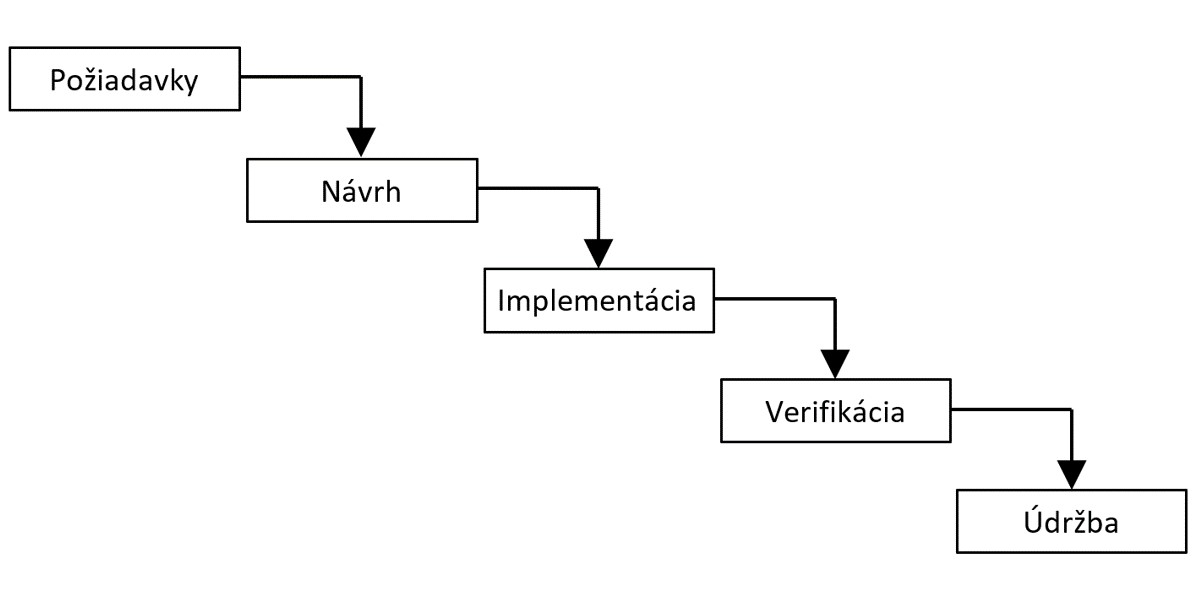
\includegraphics[scale=0.6]{vodopad1}

%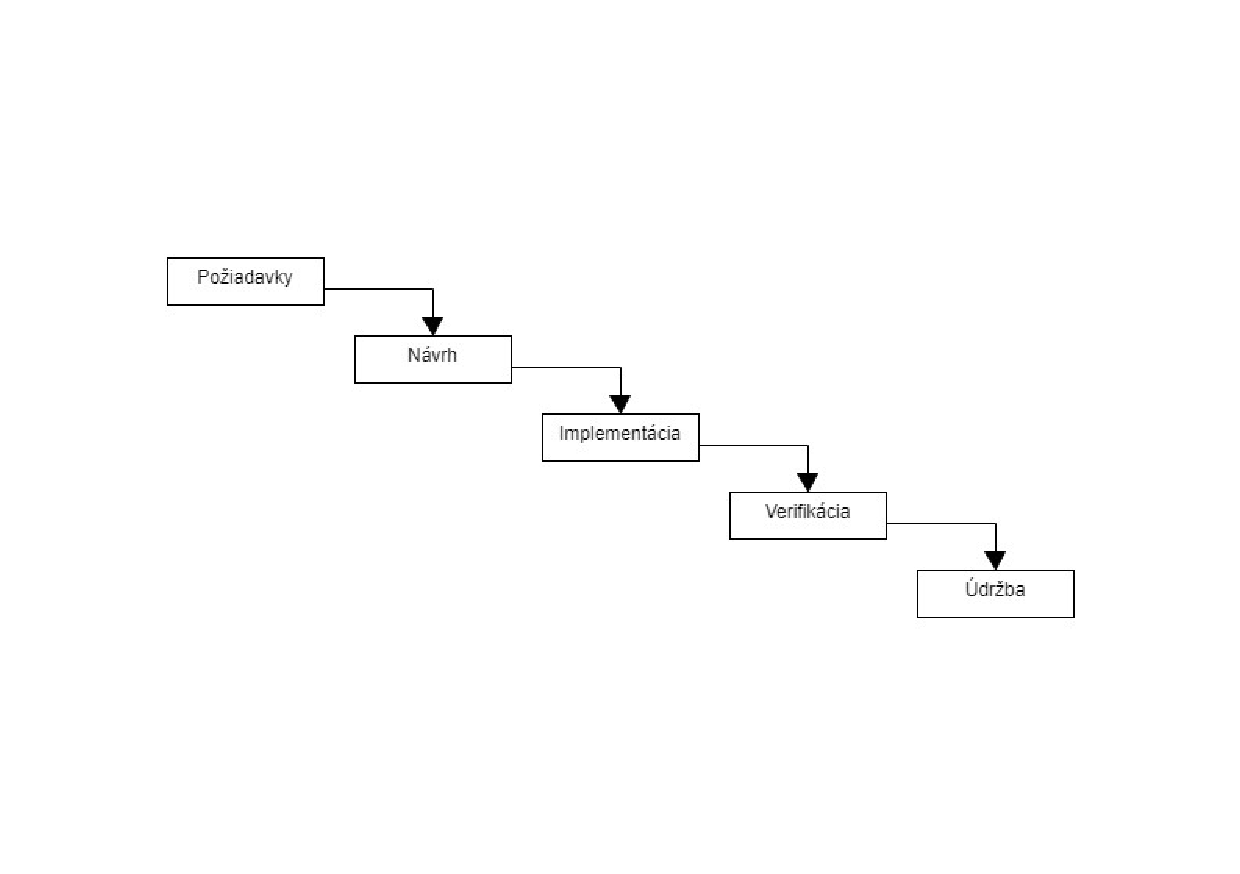
\includegraphics{vodopad} 
 
Obr.~\ref{f:rozhod} Vodopádový model tvorby softvéru.

\centering
\begin{figure*}[tbh]
Aj text môže byť prezentovaný ako obrázok. Stane sa z neho označný plávajúci objekt. Po vytvorení diagramu zrušte znak \texttt{\%} pred príkazom \verb|\includegraphics| označte tento riadok ako komentár (tiež pomocou znaku \texttt{\%}).
\caption{Rozhodujúci argument.}
\label{f:rozhod}
\end{figure*}

\subsection{Testovanie softvéru} \label{testovanie}

Základným problémom je teda\ldots{} Najprv sa pozrieme na nejaké vysvetlenie (časť~\ref{ina:nejake}), a potom na ešte nejaké %(časť~\ref{ina:nejake}).\footnote{Niekedy môžete potrebovať aj poznámku pod čiarou.}

Môže sa zdať, že problém vlastne nejestvuje\cite{Coplien:MPD}, ale bolo dokázané, že to tak nie je~\cite{Czarnecki:Staged, Czarnecki:Progress}. Napriek tomu, aj dnes na webe narazíme na všelijaké pochybné názory\cite{PLP-Framework}. Dôležité veci možno \emph{zdôrazniť kurzívou}.

\section{Umelá inteligencia}\label{AI}

Niekedy treba uviesť zoznam:

\begin{itemize}
\item jedna vec
\item druhá vec
	\begin{itemize}
	\item x
	\item y
	\end{itemize}
\end{itemize}

Ten istý zoznam, len číslovaný:

\begin{enumerate}
\item jedna vec
\item druhá vec
	\begin{enumerate}
	\item x
	\item y
	\end{enumerate}
\end{enumerate}

\section{Softvér používajúci umelú inteligenciu} \label{AISW}

\paragraph{Veľmi dôležitá poznámka.}
Niekedy je potrebné nadpisom označiť odsek. Text pokračuje hneď za nadpisom.

\section{Používanie AI pri tvorbe SW} \label{pouzitie AI pri SW}

kafnisajklmkdfs,


\section{Záver} \label{zaver} % prípadne iný variant názvu

%\acknowledgement{Ak niekomu chcete poďakovať\ldots}

% týmto sa generuje zoznam literatúry z obsahu súboru literatura.bib podľa toho, na čo sa v článku odkazujete
\bibliography{literatura}
\bibliographystyle{plain} 
\end{document}
